% vim: set spell spelllang=es syntax=tex :

\documentclass[11pt,a4paper,spanish]{beamer}

\usepackage[spanish]{babel}

\usepackage[utf8]{inputenc}

\usepackage{graphicx}

\usepackage{subcaption} %Para Subfigure

\usepackage{caption} %Para captions en las figuras sin prefijo

\usepackage{ccicons}

\usepackage{url}

\usepackage{babelbib}

\usepackage{textcomp}

\usepackage{styles/egyptian}

\newcommand{\aprox}{\raisebox{0.5ex}{\texttildelow}}
\newcommand{\bit}{\textbf{b}}
\newcommand{\Byte}{\textbf{B}}

\usefonttheme{serif}

\setlength{\parskip}{1.5mm}

\usetheme{Rochester}
\usecolortheme{whale}

%\usetheme{Warsaw}

\beamertemplatenavigationsymbolsempty

\setbeamertemplate{background canvas}{
    \raisebox{-0.99\paperheight}[0pt][0pt]{
        \makebox[\paperwidth]{
            \null
            \hspace{-1em}
            
\includegraphics[width=0.09\paperwidth]{logos/fai.pdf}
            \hspace{0.8\paperwidth}
            \hspace{-0.5em}
            \includegraphics[width=0.09\paperwidth]{logos/uncoma.pdf}
            }
    }
}

\defbeamertemplate{footline}{centered page number}
{
    \hspace*{\fill}
    \usebeamercolor[fg]{blue}
    \usebeamerfont{page number in head/foot}
    \insertpagenumber\,/\,\insertpresentationendpage
    \hspace*{\fill}\vskip2pt
}
\setbeamertemplate{footline}[centered page number]

\title{Representación de la información:\\
Unidades de información}
\author{}
\date{}

\begin{document}

\begin{frame}[noframenumbering]


    \maketitle
    \centering
    %\vspace{-8em}~
    %\begin{figure}
    %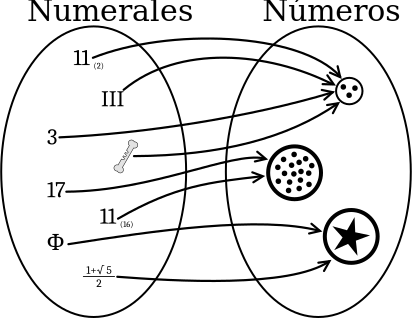
\includegraphics[height=0.65\textheight]{img/numerales.pdf}
        %\captionsetup{textfont=tiny,labelformat=empty,justification=centering}
        %\caption{}
    %\end{figure}

\end{frame}

\begin{frame}

    \frametitle{Temario}

\begin{itemize}

    \item La unidad mínima de información, el bit:
    \begin{itemize}
        \item 1 o 0, Verdadero o Falso, Sí o No.
        \item ¿Cómo representamos información más compleja?
    \end{itemize}

    \item Agrupando bits: el Byte.

    \item Múltiplos del bit y el byte:
    \begin{itemize}
        \item Prefijo del Sistema Internacional (decimal).
        \item Prefijo Binario.
    \end{itemize}

\end{itemize}
\end{frame}

\begin{frame}

\frametitle{El bit}

\begin{itemize}
    \item La mínima unidad de información.
    %\item \emph{``La información que se recibe al especificar una de dos alternativas
        %igualmente probables''} (Teoría de la Información).
    \item La respuesta a la pregunta más simple posible.
    \item Dos valores posibles:
        \begin{itemize}
            \item Verdadero o Falso.
            \item Sí o No.
            \item 0 o 1.
            \item Voltaje bajo o Voltaje alto.
        \end{itemize}
    \item Abreviado \bit{} (minúscula).
\end{itemize}
\end{frame}

\begin{frame}

\frametitle{El bit}
\framesubtitle{¿Cómo representamos información más compleja?}

\begin{minipage}{0.80\textwidth}
    ¿Cómo podríamos saber el estado de un semáforo utilizando solo preguntas
    \emph{Sí/No}?
\end{minipage}
~
\begin{minipage}{0.15\textwidth}
    \begin{figure}
    \centering
        
\includegraphics[height=0.5\textheight]{img/semaforo-off.pdf}
        \captionsetup{textfont=tiny,labelformat=empty}
        \caption{}
    \end{figure}
\end{minipage}

\end{frame}

\begin{frame}

\frametitle{El bit}
\framesubtitle{¿Cómo representamos información más compleja?}

\begin{figure}
\centering
    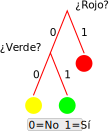
\includegraphics[height=0.9\textheight]{img/semaforo-sino.pdf}
    \captionsetup{labelformat=empty}
    \caption{}
\end{figure}

\end{frame}

\begin{frame}

\frametitle{El bit}
\framesubtitle{¿Cómo representamos información más compleja?}

\begin{minipage}{0.3\textwidth}
    \begin{figure}
        \centering
        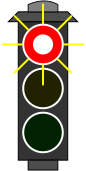
\includegraphics[height=0.5\textheight]{img/semaforo-r.pdf}
        \captionsetup{labelformat=empty}
        \caption{1}
    \end{figure}
\end{minipage}
~
\begin{minipage}{0.3\textwidth}
    \begin{figure}
        \centering
        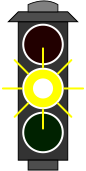
\includegraphics[height=0.5\textheight]{img/semaforo-y.pdf}
        \captionsetup{labelformat=empty}
        \caption{00}
    \end{figure}
\end{minipage}
~
\begin{minipage}{0.3\textwidth}
    \begin{figure}
        \centering
        
\includegraphics[height=.5\textheight]{img/semaforo-g.pdf}
        \captionsetup{labelformat=empty}
        \caption{01}
    \end{figure}
\end{minipage}

\end{frame}

\begin{frame}

\frametitle{El bit}
\framesubtitle{¿Cómo representamos información más compleja?}

    Alternativamente, podemos usar dos bits y asignar la correspondencia de forma
    arbitraria:

\centering
\begin{tabular}{c | c}
    Codificación & Color \\
    \hline
    00 & \hbox{\color{red}\scalebox{1.5}{$\bullet$}} \\
    01 & \hbox{\color{yellow}\scalebox{1.5}{$\bullet$}} \\
    10 & \hbox{\color{green}\scalebox{1.5}{$\bullet$}} \\
    11 & - \\
\end{tabular}

\end{frame}

\begin{frame}

\frametitle{El bit}
\framesubtitle{¿Cómo representamos información más compleja?}

    Para representar $N$ estados distintos se necesitan $\lceil{log_{2}(N)\rceil} =
    k$ bits.
    
    O dicho de otra manera: \emph{Se necesitan $k$ bits, donde $k$ es el
    entero más chico tal que $2^k\ge{}N$.}

    \pause
    Ejemplos:
    \begin{itemize}
        \item Para representar 16 colores distintos hace falta sólo: \pause
            4\bit. \pause
    \item Para representar las letras \emph{A-Z} del ingles, solo en
        mayúscula, más los dígitos decimales y otros 10 símbolos auxiliares
            (44 símbolos en total) se necesitan: \pause 6\bit. \pause
        \item Si queremos representar los números del -100 al 100 (201 en
            total), necesitamos: \pause 8\bit.
    \end{itemize}

\end{frame}

\begin{frame}

\frametitle{El bit}
\framesubtitle{Representación de enteros sin signo (positivos)}

    Si tenemos $k$ bits y queremos representar sólo enteros positivos ¿Qué
    rango de números podemos representar?

    \pause
    \begin{itemize}
        \item con $k$\bit{} podemos representar $2^{k}$ números distintos.
            \pause
        \item Como queremos incluir el cero (y queremos representar todos los
            enteros en el rango) el último número no puede ser $2^{k}$, sino
            $(2^{k})-1$. \pause
        \item Por lo tanto el \emph{Rango de Representación} de los enteros
            sin signo con $k$\bit{} es $[0,(2^{k})-1]$.\pause
        \item Para representar cada número usamos su representación binaria,
            completando con ceros a la izquierda para utilizar todos los
            \emph{bits}.
    \end{itemize}
\end{frame}

\begin{frame}

\frametitle{El bit}
\framesubtitle{Representación de enteros positivos}

    Ejemplos:
    \begin{itemize}
        \item Con 2\bit{} podemos representar el rango $[0,3]$:
        \begin{tabular}{c r c}
            Dec. & {\centering Bin.} & 2\bit\\
            0 & 0 & 00\\ \hline
            1 & 1 & 01\\ \hline
            2 & 10 & 10\\ \hline
            3 & 11 & 11\\
        \end{tabular}\pause
    \item Con 4\bit{} podemos representar el rango $[0,15]$.
    \item Con 16\bit{} podemos representar el rango $[0,65535]$.
    \item Con 32\bit{} podemos representar el rango $[0,4294967295]$.
    \end{itemize}

\end{frame}

\begin{frame}

\frametitle{El bit}
\framesubtitle{Representación de enteros positivos}

    Ejemplo:
    \begin{itemize}
        \item Con 4\bit{} podemos representar el rango $[0,7]$:
        \begin{tabular}{c r c}
            Dec. & {\centering Bin.} & 3\bit\\
            0 &   0 & 000\\ \hline
            1 &   1 & 001\\ \hline
            2 &  10 & 010\\ \hline
            3 &  11 & 011\\ \hline
            4 & 100 & 100\\ \hline
            5 & 101 & 101\\ \hline
            6 & 110 & 110\\ \hline
            7 & 111 & 111\\
        \end{tabular}
    \end{itemize}

\end{frame}

\begin{frame}
\frametitle{El bit}

Para pensar:

\begin{itemize}
    \item Si una imagen tiene una altura de 1024\emph{px}, un ancho de
        720\emph{px}, y cada pixel puede tener 1 de $16\,000$ colores
        distintos ¿Cuántos bits se necesitan para representar la imagen?
    \item ¿Cuántos bits necesito para poder representar la edad de una
        persona?
\end{itemize}

\end{frame}

\begin{frame}

\frametitle{El Byte}

    \begin{itemize}
        \item Conjunto ordenado de \textbf{bits}: Actualmente 8\bit.
        \item Unidad mínima referenciable de la memoria.
        \item Abreviado \Byte{} (mayúscula).
    \end{itemize}
    \pause

    Con un byte se puede representar:

    \begin{itemize}
        \item Números enteros del 0 al 255, o del -128 al 127.
        \item 256 colores distintos.
        \item Caracteres de letras, números, otros símbolos y secuencias de
            control.
    \end{itemize}

\end{frame}

\begin{frame}

\frametitle{El Byte}
\framesubtitle{ASCII (1963)}

\begin{itemize}
    \item 95 símbolos imprimibles y 33 caracteres de control: 128 en total.
    \item Desarrollado para usar sólo 7 bits.
    \item El bit sobrante se utilizo para crear extensiones. Actualmente es
        usa en el \emph{UTF-8}.
\end{itemize}

\end{frame}

\begin{frame}[fragile]

\frametitle{El Byte}
\framesubtitle{ASCII (1963)}
\textbf{Tabla \emph{ASCII}:}

\tiny
\begin{verbatim}
Dec Hex    Dec Hex    Dec Hex  Dec Hex  Dec Hex  Dec Hex   Dec Hex   Dec Hex
  0 00 NUL  16 10 DLE  32 20    48 30 0  64 40 @  80 50 P   96 60 `  112 70 p
  1 01 SOH  17 11 DC1  33 21 !  49 31 1  65 41 A  81 51 Q   97 61 a  113 71 q
  2 02 STX  18 12 DC2  34 22 "  50 32 2  66 42 B  82 52 R   98 62 b  114 72 r
  3 03 ETX  19 13 DC3  35 23 #  51 33 3  67 43 C  83 53 S   99 63 c  115 73 s
  4 04 EOT  20 14 DC4  36 24 $  52 34 4  68 44 D  84 54 T  100 64 d  116 74 t
  5 05 ENQ  21 15 NAK  37 25 %  53 35 5  69 45 E  85 55 U  101 65 e  117 75 u
  6 06 ACK  22 16 SYN  38 26 &  54 36 6  70 46 F  86 56 V  102 66 f  118 76 v
  7 07 BEL  23 17 ETB  39 27 '  55 37 7  71 47 G  87 57 W  103 67 g  119 77 w
  8 08 BS   24 18 CAN  40 28 (  56 38 8  72 48 H  88 58 X  104 68 h  120 78 x
  9 09 HT   25 19 EM   41 29 )  57 39 9  73 49 I  89 59 Y  105 69 i  121 79 y
 10 0A LF   26 1A SUB  42 2A *  58 3A :  74 4A J  90 5A Z  106 6A j  122 7A z
 11 0B VT   27 1B ESC  43 2B +  59 3B ;  75 4B K  91 5B [  107 6B k  123 7B {
 12 0C FF   28 1C FS   44 2C ,  60 3C <  76 4C L  92 5C \  108 6C l  124 7C |
 13 0D CR   29 1D GS   45 2D -  61 3D =  77 4D M  93 5D ]  109 6D m  125 7D }
 14 0E SO   30 1E RS   46 2E .  62 3E >  78 4E N  94 5E ^  110 6E n  126 7E ~
 15 0F SI   31 1F US   47 2F /  63 3F ?  79 4F O  95 5F _  111 6F o  127 7F DEL
\end{verbatim}

\end{frame}

\begin{frame}

\frametitle{El Byte}
\framesubtitle{ASCII (1963)}

    Representando ``IC 2023'' en \emph{ASCII}:

\centering
\begin{tabular}{c  c  c}
    I & 49 & 0100 1001\\ \hline
    C & 43 & 0100 0011\\ \hline
      & 20 & 0010 0000\\ \hline
    2 & 32 & 0011 0010\\ \hline
    0 & 30 & 0011 0000\\ \hline
    2 & 32 & 0011 0010\\ \hline
    3 & 33 & 0011 0011\\
\end{tabular}

\end{frame}

\begin{frame}

\frametitle{Múltiplos del bit y el byte}

    \framesubtitle{Prefijo del Sistema Internacional (decimal)}

Para el Byte:

\centering
\begin{tabular}{l l l}
    Kilobyte & $1\,000^{1}$ bytes & \textbf{kB}\\ \hline
    Megabyte & $1\,000^{2}$ bytes & \textbf{MB}\\ \hline
    Gigabyte & $1\,000^{3}$ bytes & \textbf{GB}\\ \hline
    Terabyte & $1\,000^{4}$ bytes & \textbf{TB}\\ \hline
    Petabyte & $1\,000^{5}$ bytes & \textbf{PB}\\ \hline
    Exabyte & $1\,000^{6}$ bytes & \textbf{EB}\\ \hline
    Zettabyte & $1\,000^{7}$ bytes & \textbf{ZB}\\ \hline
    Yottabyte & $1\,000^{8}$ bytes & \textbf{YB}\\
\end{tabular}

\end{frame}

\begin{frame}

\frametitle{Múltiplos del bit y el byte}

    \framesubtitle{Prefijo del Sistema Internacional (decimal)}

Para el bit:

\centering
\begin{tabular}{l l l}
    Kilobit & $1\,000^{1}$ bits & \textbf{kb}\\ \hline
    Megabit & $1\,000^{2}$ bits & \textbf{Mb}\\ \hline
    Gigabit & $1\,000^{3}$ bits & \textbf{Gb}\\ \hline
    Terabit & $1\,000^{4}$ bits & \textbf{Tb}\\ \hline
    Petabit & $1\,000^{5}$ bits & \textbf{Pb}\\ \hline
    Exabit & $1\,000^{6}$ bits & \textbf{Eb}\\ \hline
    Zettabit & $1\,000^{7}$ bits & \textbf{Zb}\\ \hline
    Yottabit & $1\,000^{8}$ bits & \textbf{Yb}\\
\end{tabular}
\end{frame}

\begin{frame}

\frametitle{Múltiplos del bit y el byte}

\framesubtitle{Prefijo Binario}

\centering
\begin{tabular}{l l l}
    Kibibyte & $1\,024^{1}$ bytes & \textbf{kiB}\\ \hline
    Mebibyte & $1\,024^{2}$ bytes & \textbf{MiB}\\ \hline
    Gibibyte & $1\,024^{3}$ bytes & \textbf{GiB}\\ \hline
    Tebibyte & $1\,024^{4}$ bytes & \textbf{TiB}\\ \hline
    Pebibyte & $1\,024^{5}$ bytes & \textbf{PiB}\\ \hline
    Exbibyte & $1\,024^{6}$ bytes & \textbf{EiB}\\ \hline
    Zebibyte & $1\,024^{7}$ bytes & \textbf{ZiB}\\ \hline
    Yobibyte & $1\,024^{8}$ bytes & \textbf{YiB}\\
\end{tabular}

\tiny ($1024 = 2^{10}$)
\end{frame}

\begin{frame}

\frametitle{Múltiplos del bit y el byte}

\framesubtitle{Usos y confusiones}

El prefijo binario es estándar desde el 1998, antes de eso se utilizaban los
    mismos nombres para referirse a cantidades múltiplo de $1\,000$ y
    $1\,024$. A cual de las dos se hacia referencia debía deducirse del
    contexto. Todavía la costumbre persiste.

\pause
Usos comunes del prefijo decimal:

\begin{itemize}
    \item Las velocidades de transmisión suelen medirse en múltiplos decimales del bit.
    \item Los tamaños de los discos duros se comunican en múltiplos decimales
        del byte.
\end{itemize}

\pause
Usos comunes del prefijo binario:

\begin{itemize}
    \item El tamaño de las memorias principales \emph{(RAM)}.
    \item El tamaño de los archivos en el disco (aunque algunos sistemas
        utilicen la nomenclatura incorrecta).
\end{itemize}

\end{frame}

\begin{frame}

\frametitle{Múltiplos del bit y el byte}

\framesubtitle{Usos y confusiones}

Para pensar:

\begin{itemize}
    \item Si compro un disco de 2\emph{TB} ¿Cuántos \emph{TiB} de datos puedo
        almacenar en el?
    \item Si mi conexión es de 1\emph{Mb/s} ¿Cuál es la velocidad en
        \emph{MiB/s}?
    \item Si una imagen tiene una altura de 1024\emph{px}, un ancho de
        720\emph{px}, y cada pixel puede tener 1 de $16\,000$ colores
        distintos ¿Cuántos KiB se necesitan para representar la imagen?
\end{itemize}

\end{frame}

\begin{frame}

    \frametitle{Temario}

\begin{itemize}

    \item La unidad mínima de información, el bit:
    \begin{itemize}
        \item 1 o 0, Verdadero o Falso, Sí o No.
        \item ¿Cómo representamos información más compleja?
    \end{itemize}

    \item Agrupando bits: el Byte.

    \item Múltiplos del bit y el byte:
    \begin{itemize}
        \item Prefijo del Sistema Internacional (decimal).
        \item Prefijo Binario.
    \end{itemize}

\end{itemize}
\end{frame}

\begin{frame}

\title{¿Consultas?}
\maketitle

\end{frame}

\newcounter{lastPage}
\setcounter{lastPage}{\number\value{page}}

\setcounter{page}{\number\value{lastPage}}

\end{document}
